\documentclass{article}

% if you need to pass options to natbib, use, e.g.:
% \PassOptionsToPackage{numbers, compress}{natbib}
% before loading nips_2016
%
% to avoid loading the natbib package, add option nonatbib:
% \usepackage[nonatbib]{nips_2016}

\usepackage[nonatbib,final]{nips_2016} % produce camera-ready copy
% to compile a camera-ready version, add the [final] option, e.g.:
% \usepackage[final]{nips_2016}

\usepackage[utf8]{inputenc} % allow utf-8 input
\usepackage[T1]{fontenc}    % use 8-bit T1 fonts
\usepackage{hyperref}       % hyperlinks
\usepackage{url}            % simple URL typesetting
\usepackage{booktabs}       % professional-quality tables
\usepackage{amsfonts}       % blackboard math symbols
\usepackage{nicefrac}       % compact symbols for 1/2, etc.
\usepackage{microtype}      % microtypography
\usepackage{blindtext}
\usepackage{graphicx}       %insert graph
\usepackage{epstopdf}       %insert graph .esp

\usepackage[sorting=none]{biblatex}
\addbibresource{progress.bib}
\title{Predicting Cuisines and Recommendation on Recipes}

% The \author macro works with any number of authors. There are two
% commands used to separate the names and addresses of multiple
% authors: \And and \AND.
%
% Using \And between authors leaves it to LaTeX to determine where to
% break the lines. Using \AND forces a line break at that point. So,
% if LaTeX puts 3 of 4 authors names on the first line, and the last
% on the second line, try using \AND instead of \And before the third
% author name.

\author{
  Zitian Wang\\
  s1882252\\
  \texttt{s1882252@ed.ac.uk} \\
  %% examples of more authors
  \And
  Siyu Zhou\\
  s2057647\\
  \texttt{s2057647@ed.ac.uk} \\
 \And
  Xingjian Lu\\
  s2014340\\
  \texttt{s2014340@ed.ac.uk} \\
 \And
  Yijin Zhang\\
  s2114888\\
  \texttt{s2114888@ed.ac.uk}\\
}

\begin{document}

\maketitle

\begin{abstract}
 With the springing up of recipe sharing and recommendation platforms, how to classify recipes into cuisines has been an essential problem to deal with for every platform. Also, users need recommendations when they only have a partial recipe. In this project, we first study the existing dataset with 4236 recipes from 12 cuisines in Exploratory Data Analysis to find out its distribution and similarity. We then discovered that the best model to predict the cuisines is Logistic Regression with a test accuracy of 80.0\%. For the partial recipe filling, item-based PCA is the best algorithm, providing a precision of 69.7\% at a data missing rate of 2\%.
\end{abstract}

\section{Introduction}
\subsection{Description of the task/objective}

Given a list of ingredients in recipes, it is the aim of this project to firstly predict the cuisines (Chinese/Japanese/Italian,...,etc) the recipes are from, and secondly if given partial recipes, suggest the missing ingredients. The report begins with summarizing the relevant background and previous work, followed by exploratory data analysis on the data set available, and then introduces both the recipe prediction and partial recipe filling (recommendation system with collaborative filtering) algorithms. 

\subsection{Relevant background and related previous work}
A number of papers have looked into the prediction of cuisines based on ingredients. Ghewari et al.
\cite{ghewari2015predicting} 
used a multi-class Support Vector Classifier to predict the cuisine based on the ingredients; they reached a validation accuracy of 0.8132 and test accuracy of 0.7823. The performance of different classifiers were also compared in the paper, and SVM turned out to have the highest accuracy. Jayaraman et al.
\cite{jayaraman2017analysis} 
analysed the correlation between recipes and the ingredients with SVM and associative classification; they also compared different classifiers (Multinomial Logistic Regression, Random Forest,...,etc) and agreed with Ghewari et al. that support vector classifiers is the most accurate among all studied with an accuracy of approximately 80\%. Kumar et al.
\cite{kumar2016cuisine}
introduced a method of cuisine prediction based on ingredients using tree boosting algorithms; their XG-Boosting algorithm also obtained an accuracy of about 80\% for cuisine prediction, which is consistent with the previous studies.

Besides, several studies also look into the collaborative filtering algorithm that we may use in completing the partial recipes. Su et al.
\cite{su2009survey}
provided a review for collaborative filtering techniques. The research by Sarwar et al.
\cite{sarwar2001item}
analysed different item-based recommendation generation algorithms and suggested that the performance they provide is dramatically better than user-based algorithms. Wang et al.
\cite{wang2006unifying}
used similarity fusion to unify the user-based and item-based collaborative filtering approaches, achieving a more robust model to data sparsity.

Moreover, as a classic example of collaborative filtering, movie recommendation has been the subject of numerous researches. Jing Li et al.
\cite{bridge}
proposed a way of dealing with the sparse data set, and the prediction results based on cosine similarities outperforms some existing collaborative filtering algorithms. Sang-min Choi et al
\cite{genre}
came up with a movie recommendation system based on genre correlations. Their way of similarity calculation resembles the item-based cosine similarities, which all use the same idea as nearest-neighbors techniques. Koren et al
\cite{Koren2009}
proposed a collaborative filtering technique for recommender systems with matrix factorization, which outperforms the nearest-neighbors techniques.

However, since none of the movie ratings they are dealing with is binary, we have to combine their ideas and the ways of treating binary data set in our project. Verstrepen et al.
\cite{cf_method1}
provided an overview on dealing with binary, positive-only data in collaborative filtering. Lai et al.
\cite{cf_method2}
proposed an algorithm in binary user preference prediction problem that requires to separate for a given user, the tracks with high ratings, from those unrated ones. They gained a final error rate of 2.4808\%. Those are methods we can look into and learn from in this project.

Also, for the performance measurement of the binary data prediction, the system of accuracy, sensitivity, specificity and precision is used in the research of Kumar et al.
\cite{metrics}
as performance measures. We will continue to use this evaluation metrics as the performance can be assessed in different aspects. 

\subsection{Explanation of the significance/relevance of the objective/task}
What to eat and how to cook has been one of people's major daily concerns. The springing up recipe sharing and recommendation platforms call for better classification of recipes to provide people with more suitable recommendations. Also, while users may already in possession of or have preferences on certain ingredients, a recipe completion system is also needed to suggest what to cook and what is still needed to complete the feast. On completing this project, we hope to give more insights into these two problems and if possible, bring practical improvements to people's everyday lives.

\section{Data preparation and Exploratory data analysis}
The Cuisines Recipes data set contains a total of 4236 recipes, each from one cuisine, with a total of 12 different cuisines, each containing 353 recipes. Each recipe is associated with a specific set of ingredients, and 709 different ingredients in total.

The top 10 ingredients used in all cuisines are shown in  \autoref{fig:Ingredient distribution over cuisines}, sort according to the frequency. It can be seen that garlic and onion are the two most popular ingredients, which are used in more than half of all recipes. The top three ingredients used in different cuisines are tabulates in \emph{\textbf{table}}~\ref{popular ingredients in each cuisine}, for East Asian countries, e.g., China, Japan, Thailand, sauce (including soy sauce and fish sauce) is most popular. While for continental European countries, such as England, France, Germany, etc., butter and onion are most used. Furthermore, garlic is a popular ingredient all around the world, which is not restricted by region. In addition, the number of different ingredients in each cuisine is shown in  \emph{\textbf{table}}~\ref{The number of different ingredients in each cuisine}, showing that the number is mostly between 250 and 300 and there is no significant difference.

\begin{figure}[ht]
\vskip -4mm
\centering
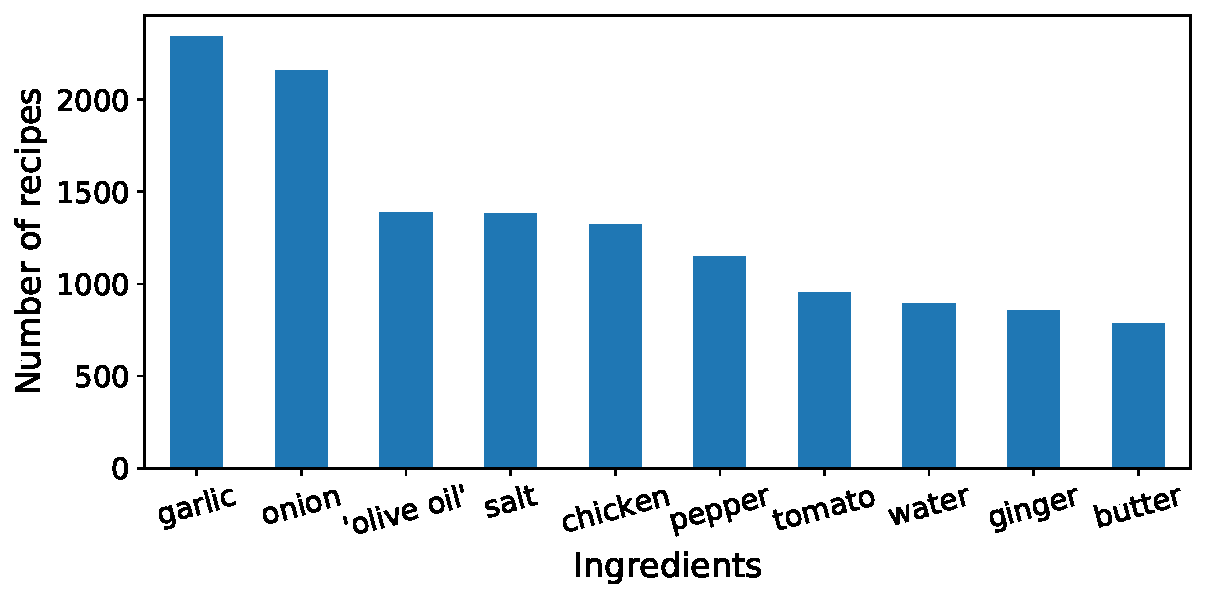
\includegraphics[width=3.5in]{DME-template/Figure/Ingredient distribution over cuisines.pdf}
\vskip -4mm
\caption{Ingredient distribution over cuisines.}
\label{fig:Ingredient distribution over cuisines} 
\end{figure}

\begin{table}[htb]
\vskip -3mm
\begin{center}
\begin{tabular}{lcccc}
\hline
Cuisines &  & ingredients \\
\hline
Chinese & soy sauce & garlic & ginger \\
English & onion & butter & potato \\
French & garlic & butter & wine \\
German & onion & pepper & salt \\
Greek & olive oil & garlic & onion \\
Indian & onion & garlic & ginger \\
Italian & garlic & olive oil & parmesan cheese \\
Japanese & soy sauce & rice wine & sugar \\
Mexican & onion & tortilla & garlic \\
Moroccan & onion & garlic & olive oil \\
Spanish & garlic & olive oil & onion \\
Thai & garlic & fish sauce & chicken \\
\hline
\end{tabular}
\vskip 0.5mm
\caption{The most popular ingredients in each cuisine.}
\label{popular ingredients in each cuisine}
\end{center}
\vskip -9mm
\end{table}

\begin{table}[htb]
\vskip 2mm
\begin{center}
\begin{tabular}{lccccc}
\hline
Chinese & English & French & German & Greek & Indian\\
240 & 317 & 292 & 263 & 260 & 235\\
\hline
Italian & Japanese & Mexican & Moroccan & Spanish & Thai\\
249 & 286 & 250 & 254 & 277 & 260\\
\hline
\end{tabular}
\vskip 1mm
\caption{The number of different ingredients in each cuisine.}
\label{The number of different ingredients in each cuisine}
\end{center}
\vskip -9mm
\end{table}

In order to realize the visualization of data, we have tried a variety of dimension reduction methods to reduce the data to two dimensions. Through comparison, it shows that the best visualization performance can be obtained by using ISOMAP (neighbors=3), and the scatter plots are shown in \autoref{fig:Scatter plot for all Cuisines} and \autoref{fig:Scatter plot for two part Cuisines}, each point represents a recipe.

\autoref{fig:Scatter plot for all Cuisines} shows the scatter of all cuisines. In the plot, Asian recipes are mainly concentrated on the left part of the picture, while European, Moroccan and Mexican cuisines were mainly concentrated on the right part of the plot. For further analysis, we conduct dimension reduction on these two parts respectively by using ISOMAP.

\autoref{fig:Scatter plot for two part Cuisines}.a shows the scatter plot of Asian recipes. It can be seen that Chinese and Japanese recipes (East Asian) are mainly concentrated in the lower right corner, with a large area of overlap. Thai recipes (Southeast Asia) and Indian recipes (South Asia) are mainly distributed in the upper and the lower left part respectively.

\autoref{fig:Scatter plot for two part Cuisines}.b shows the scatter plot of European, Moroccan and Mexican cuisines. We can find that the recipes in countries along the Mediterranean coast, including Greek, Italian, Moroccan and Spanish, are mainly distributed in the right half of the plot, with a large area of overlap. France is located in the core of Western Europe and is the hub of cultural communication (including food), having rich ingredients and diverse dishes, so the distribution of France recipes is very scattered, almost covering the whole plot. Britain and German (Northern Europe) recipes are mainly located in the lower left part. Mexican is in North America, but it was a colony of the Spanish Empire from 1521 to 1821, so it can be reasonably speculated that its traditional cuisine would be influenced by Europe to some extent. As can be seen from the figure, it has a great similarity with European cuisines.

Based on the visualization analysis of data dimension reduction, we can mainly draw the following two conclusions:
First, the distribution and similarity of data of different cuisines are mainly affected by geographical and historical factors. Second, the recipes in East Asia and Mediterranean regions overlap in large areas and have high similarity respectively, which poses great challenges to classification.

\begin{figure}[ht]
\vskip -5mm
\centering
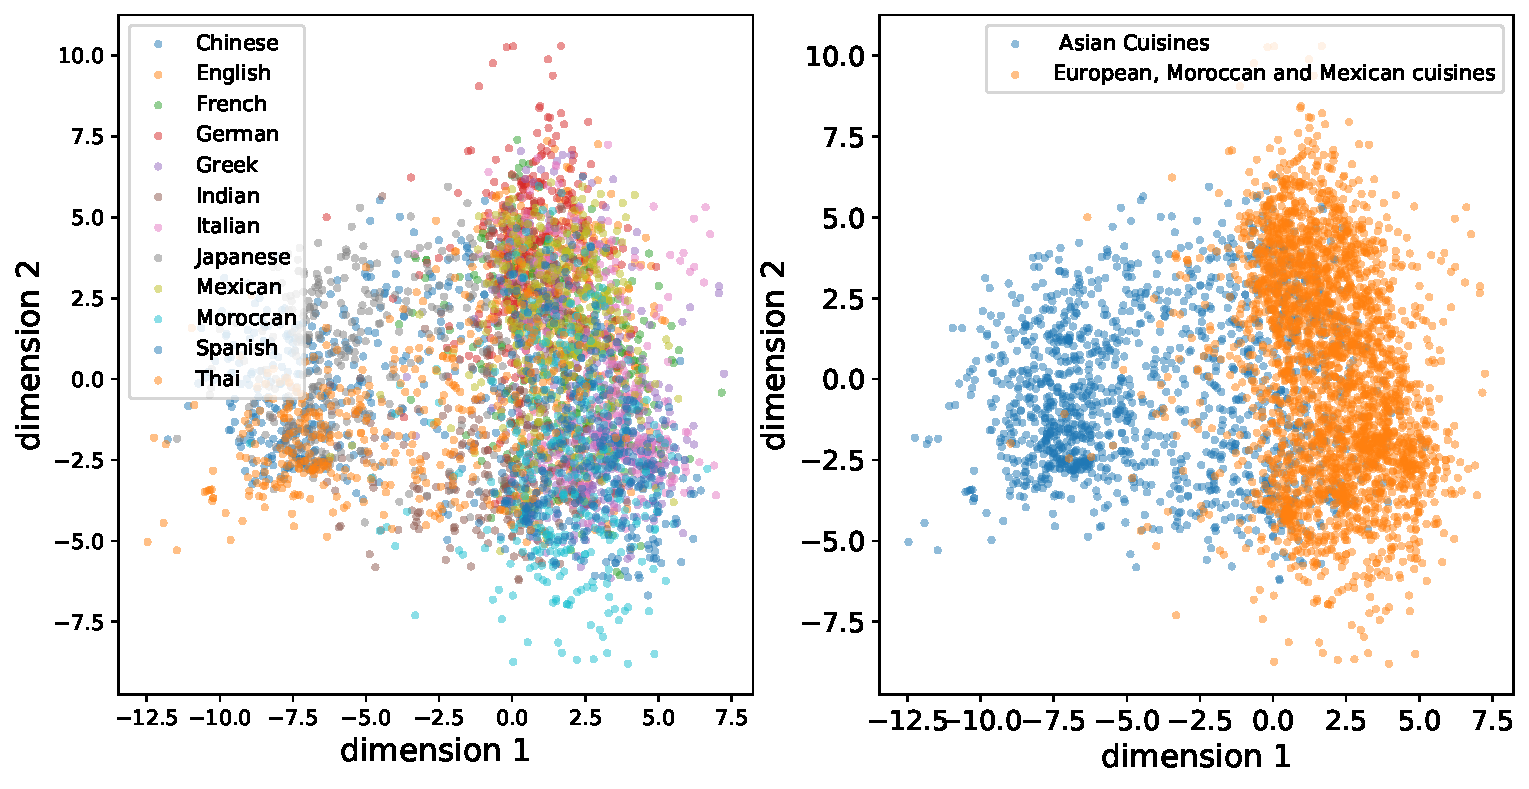
\includegraphics[width=4in]{DME-template/Figure/Scatter plot for all Cuisines.pdf}
\vskip -3mm
\caption{Scatter plot for cuisines.}
\label{fig:Scatter plot for all Cuisines} 
\vskip -3mm
\end{figure}

\begin{figure}[ht]
\vskip -1mm
\centering
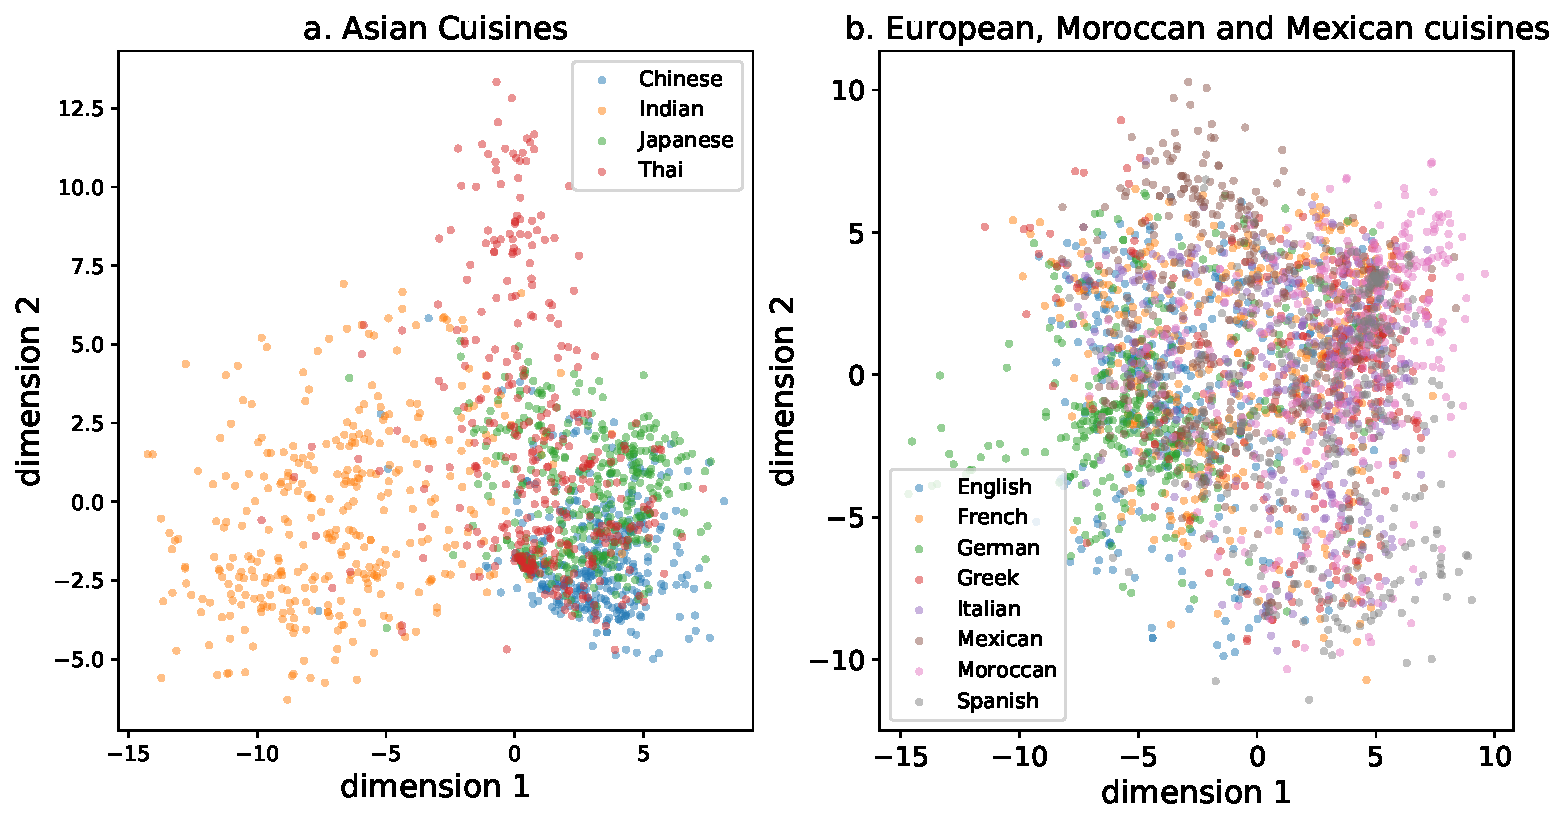
\includegraphics[width=4in]{DME-template/Figure/Scatter plot for two part Cuisines.pdf}
\vskip -3mm
\caption{Scatter plot for two different regions' cuisines.}
\label{fig:Scatter plot for two part Cuisines} 
\vskip -5mm
\end{figure}

\section{Cuisine prediction}

\subsection{Preliminary}
The aim of this task is to predict the cuisine to which a recipe belongs based on its ingredients. It can be defined as a classification problem. The input is the ingredients of a recipe, and the output is the predicted cuisine. As there are 709 different ingredients in all recipes, each recipe is denoted as a vector containing 709 elements, and each element corresponds to an ingredient. If the ingredient shows in a recipe, the value of the corresponding element in the vector is 1, otherwise 0. 

\textbf{Data split.}
%\subsubsection{Data split}
For this dataset, we employ the "training-validation-test" data split, where the training set is for training, the validation set is for hyper-parameters choosing, and the test set is for testing the generalization ability of the model. First, the dataset is shuffled and 20\% of the dataset is split as test set. The splitting is stratified and preserves the proportion of each cuisine. Second, we conduct 5-fold cross-validation to the remaining data. The remaining data is split into training set and validation set at a ratio of $4:1$. The splitting is also stratified, preserving the percentage of samples for each class. 

\textbf{Evaluation metric and Baseline.}
%\subsubsection{Evaluation metric and Baseline}
The metric we use to evaluate our models is accuracy, which is the proportion of correctly classified samples in all classified samples. As every cuisine has the same number of recipes (353 recipes), we set the 'random guess' prediction as our baseline, which means given a recipe, we randomly predict a cuisine from the 12 cuisines. The accuracy on the validation set of the 'random guess' classifier is 8.4\%.

\textbf{Overall training process.}
%\subsubsection{Overall training process}
The training process for a classifier is described as below: (1) Use the training set to train the model and fit the model with the validation set to get the validation accuracy. As we implement 5-fold cross-validation, we compute the mean validation accuracy of the 5 cases for comparison among models. (2) Alter hyper-parameters and train the corresponding models, and get the validation accuracy of the models. (3) Select the model with the highest validation accuracy. (4) Train the selected model using the combination of training set and test set. (5) Fit the model with the test set and get test accuracy.

\subsection{Classifiers and Implementation}
\textbf{Support Vector Machines (SVM).}
SVM is to find a hyperplane that maximize the margin. This method can deal with both linear classification and non-linear classification. For linear SVM, we use different values of penalty parameter C of the error term, and get the highest validation accuracy when C is 0.08. For non-linear SVM, we use the radial basis function kernel (RBF kernel), and we get the highest validation accuracy when C is 2.0. We use the C that brings the highest validation accuracy to train our final SVM model.

\textbf{Logistic Regression.}
For Logistic Regression, we use the stochastic Average Gradient descent to solve the optimization problem, which is denoted as solver 'sag' in Scikit-learn. And the penalty parameter C of the error term we set is 0.5, which brings the best validation accuracy.

\textbf{Decision Tree.}
For Decision Tree classifier, we use Gini impurity to measure the quality of a split. And to mitigate over-fitting, the max depth of the tree is set to 45, which brings the best validation accuracy.

\textbf{K-Nearest Neighbor (KNN).}
KNN is to predict the result based on the Neighbors of the given data. For KNN, the value of K is set to 20, which brings the highest validation accuracy. And the metric for distance is Euclidean metric.

\textbf{Extreme Gradient Boosting (XGBoost).}
XGBoost employs tree learning under the gradient boosting algorithm. The number of estimator is set to 40, which brings the highest validation accuracy. And the learning rate is 0.3, the max depth is 10.

\textbf{Multi-layer Perceptron classifier (MLP).}
MLP classifier can be seen as simple neuron networks with several fully connected layers. The MLP classifier we use has 3 hidden layers, whose size are 512, 128, 24 respectively. The batch size is 200. The solver for weight optimization is stochastic gradient descent. The activation function is Rectified Linear Unit (ReLU). To alleviate over-fitting, the early stop strategy is used.

\subsection{Results for cuisine prediction}
The accuracy results of the classifiers are shown in \emph{\textbf{table}}~\ref{acc}. From the results, we can see all the classifiers we implement perform much better than the ’random guess’ baseline. The Logistic Regression classifier achieves the highest test accuracy, which is 80.0\%. Linear SVM and MLP performs almost as well as Logistic Regression. SVM with RBF kernel and XGBoost also bring good results, which are around 79\%. However, Decision Tree and KNN perform not so well. These results are similar to the results of the cuisine prediction tasks in \cite{ghewari2015predicting} \cite{jayaraman2017analysis} \cite{kumar2016cuisine} \cite{kalajdziski2018cuisine}, where SVM, Logistic Regression, XGBoost and MLP bring good results. Besides, it is worth noting that the Logistic Regression model is not as complex as SVM with RBF kernel, XGBoost and MLP, but it outperforms them. It can be explained that SVM with RBF kernel, XGBoost and MLP has the training accuracy of above 97\%, which means they suffer from over-fitting and indicates the three models may be too complex for this dataset. And the training accuracy of the Logistic Regression model is 88.4\%, which means the extent of over-fitting is acceptable and much lower than those three over-fitting models.

\begin{table}[htb]
\vskip -2mm
\begin{center}
\begin{tabular}{lcccc}
\hline
Models & Test accuracy \\
\hline
'random guess' baseline &  8.4\% \\
Decision Tree & 61.9\% \\
KNN & 66.5\% \\
SVM with RBF kernel  & 78.7\% \\
XGBoost & 79.0\% \\
Linear SVM &  79.6\% \\
MLP & 79.6\% \\
Logistic Regression  & \textbf{80.0\%} \\
\hline
\end{tabular}
\vskip 0.5mm
\caption{Classification accuracy of models.}
\label{acc}
\end{center}
\vskip -5mm
\end{table}

The confusion matrix for Logistic Regression model is shown in \autoref{confusion}. From the confusion matrix, we can see that the classifier always makes mistakes when distinguishing Japanese cuisine from China Cuisine. And the classifier also sometimes makes mistakes when classifying the recipes in Mediterranean regions. These observations indicate that the recipes of Japanese cuisine and China Cuisine are similar and the recipes of Mediterranean regions are also similar, which is consistent with the analysis in the exploratory data analysis section.

\begin{figure}[ht]
\vskip -6mm
\centering
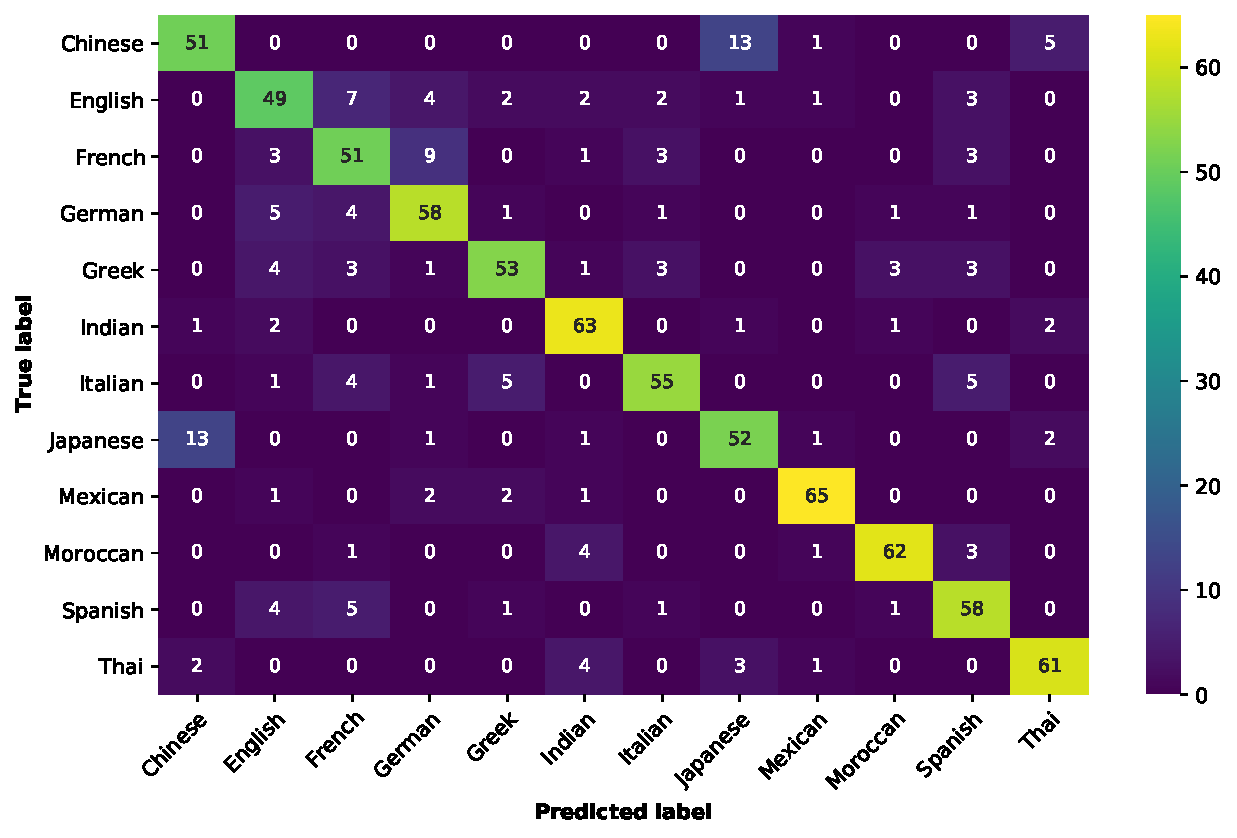
\includegraphics[width=4in]{DME-template/Figure/confu_ma.pdf}
%\includegraphics[height=2cm,width=3cm]{exp.eps}
\vskip -3mm
\caption{The confusion matrix for Logistic Regression model.}
\label{confusion} 
\vskip -9mm
\end{figure}

%\section{Results} 
\section{Collaborative Filtering}
For collaborative filtering, it is assumed at the beginning that we know which cuisine a particular recipe belongs to, as specific recipes may depend highly on cuisines. However, we only have access to partial recipes. In other words, we only know whether some but not all of the 709 ingredients are included in the recipes. It is therefore a target for us to fill in the missing parts. To create such a partial dataset, we randomly convert a certain percentage of entries into NA in every recipe. Then, we discuss and choose the baselines and metrics. To restore the complete dataset, we consider three families of collaborative filtering methods: two memory-based methods (user-based and item-based), and one model-based method (matrix factorization). The user-based methods calculate the similarity between ingredients and recommend those that are most similar to the ones known used. The item-based methods, on the other hand, calculate the similarity between recipes and recommend the ingredients used in the most similar recipes. These algorithms will be applied respectively to each of the 12 cuisines. Since all methods require a complete input dataset, we impute the missing values with a baseline before feeding it to the algorithm. Finally, the 5 methods (including two PCA version memory-based methods) and two baselines will be compared to find the best model(s). We will also discuss the effect of missing proportion in each recipe, as well as situations where the chosen algorithms don't perform well.

\subsection{Preliminary}
%\subsubsection{Simulate Dataset with missing values}
We first randomly convert 2\% of entries into NA in every recipe. The dataset whose recipes have k\% missing is denoted as “k\% partial dataset”. We compare the algorithms’ performance through the metrics which need the actual and predicted values for every NA entry. Thus, the traversing can be extremely computationally costly if a large proportion is missing. That’s why we only assume one level of missing rate, 2\% through the process of finding the most accurate model. We will still look into the effect of missing proportions at the end of the report.

%\subsubsection{Baselines}
Then, we define the baselines. The matrix is transposed so that ingredients are in rows and recipes in columns. Baseline1: user mode. The NAs are imputed as the mode for the i-th ingredient (i-th user/row mode). Baseline2: random binary numbers based on users/ingredients. The NAs are imputed as random numbers that follow a binomial distribution. The success probability is based on the frequency of occurrence for the given ingredient in the given cuisine.

%\subsubsection{Evaluation Metrics}
For evaluation, we use two metrics (sensitivity and precision) to compare the models. They are defined as follows:
$Sensitivity = \frac{TP}{TP+FN}$, $Precision = \frac{TP}{TP+FP}$
where TP, TN, FP, FN are true positive, true negative, false positive and false negative respectively. Unlike the previous study by Kumar et al.\cite{metrics}, we do not use the accuracy $\frac{TP+TN}{TP+FN+TN+FP}$ since for such a sparse matrix (only 24 out of 709 ingredients have been used in more than 10\% recipes), the accuracy is always very high even if we predict all zeros for every missing value and the accuracy doesn’t really differ between algorithms.

To compare the sensitivity and precision, we applied simulation study and generated 20 “2\% partial datasets” for the two baselines. It is discovered that the average precision of baseline1 for all 12 cuisines is about 0.608 and that of baseline2 is around 0.239. The average sensitivity of baseline1 is approximately 0.127 and that of baseline2 is about 0.242.

\subsection{Model comparison}
%\subsubsection{Imputation}
The precision of baseline1 is significantly greater than that of baseline2 although the baseline1 has lower sensitivity than baseline2. We choose baseline1 to impute the incomplete dataset.

%\subsubsection{Models}
\textbf{Memory-based models.}
The memory-based models make predictions based on the similarity matrix, which can be computed using either the complete dataset (the 2\% partial dataset imputed by the baseline1), or the PC score matrix. By applying PCA to the complete dataset that was imputed by baseline1, the features on either dimension (user-ingredients/item-recipes) are extracted to calculate the similarity on the other. The inaccuracy caused by data imputation is neutralized after PCA feature extraction. For the 4 memory-based models (user-based model, PCA user-based model, item-based model and PCA item-based model), we carry out simulation studies to find the best parameters. It is discovered that keeping 50 PC components in PCA item-based similarity calculation and 30 PC components in PCA user-based similarity calculation reveal the best results.

\textbf{Model-based models.}
After we impute the incomplete matrix with baseline1, the matrix factorization (MF) is applied to decomposing the dataset into the product of two lower-dimension rectangular matrices. We then multiply these two matrices to rebuild the original matrix and predict the NA entries based on the corresponding outcomes in the rebuilt matrix. We use 5 as the number of latent factors which were determined again by simulation studies.

%\subsubsection{Results}
\emph{\textbf{Table}}~\ref{Model comparison} shows the performance of the 5 algorithms and 2 baselines in 12 classes of cuisines. We could find that the sensitivity is not a stable metric because it varies a lot among different classes of cuisines. For example, the sensitivity varies from 0.16 to 0.55 in the user-based method. However, precision is much more stable. Therefore, we select the PCA-item based model and matrix factorization model as the best based on their outstanding performances on precision and acceptable behaviors on sensitivity. 

\begin{table}[htb]
\centering
\vskip -5mm
\begin{center}
\begin{tabular}{lcccccccc}
\hline

&Model& item-based & user-based & PCA-item & PCA-user & MF & b1 &b2\\
\hline
Sensitivity&mean & 0.28 & 0.34 & 0.22 & 0.20 & 0.22 & 0.13 & 0.24
\\
&std dev & 0.24 & 0.40 & 0.23 & 0.38 & 0.21 & 0.24 &	0.17\\
\hline
Precision&mean &0.64&0.35&0.69&0.56&0.66&0.61&0.24

\\
&std dev &0.07 &0.07 &0.10 &0.18 &0.09 &0.31 &0.18 
\\
\hline
\end{tabular}
\vskip 1mm
\caption{Model comparison. (b1 and b2 are baseline1 and baseline2)}
\label{Model comparison}
\end{center}
\vskip -8mm
\end{table}

Also, we can see that both item-based models beat the user-based models in precision. This can be understood intuitively, as user-based models recommend similar ingredients to the used ones, while item-based models recommend those used in similar recipes. In real circumstances, it’s not actually the case that we use similar ingredients in a recipe, say, both potatoes and sweet potatoes – we tend to avoid them; yet for recipes that are similar, they tend to use ingredients that work similarly.

Since the metrics are calculated from the actual and predicted values in all NA entries which require traversing, calculating the performance of 1 algorithm in 12 classes of cuisines has a high computation complexity. The results are averaged after calculating the performance metrics on 20 different NA samples to capture the randomness of partial data simulation. The number seems a bit less as is confined by running time but it is still enough to draw the conclusion.

\subsection{Effects of missing proportion}
It is already revealed, that the PCA item-based model and the matrix factorization model have comparable performances. Here we need to evaluate them in different missing rates. The metrics of the outcomes among 12 cuisines are averaged for comparison in \emph{\textbf{table}}~\ref{Performance of models}. We find that both the Precision and Sensitivity decrease slowly as the level of missing proportion goes up. Also, it is obvious that PCA-item model performs better than the MF model in all 5 levels of missing. Thus we could conclude that PCA-item model is the best.

Calculating the performace for a dataset where a large proportion, say, 50\% of entries are missing can take a very long time (it requires traversing more than a million entries in one run). It is also intuitively more inaccurate as we generally know less about the input data. Thus, we only attempted in this project a maximum missing rate of 20\%  to investigate the effect of missing proportions, as is limited by the computation time, but it is still enough for us to observe the trend.

\begin{table}[htb]
\centering
\vskip -9mm
\begin{center}
\begin{tabular}{lcccccccc}
\hline

&missing rate& 1\% & 2\% & 5\% & 10\% & 20\%\\
\hline
Matrix Factorization&Precision & 0.661 & 0.648&0.657&0.657&0.650 
\\
&Sensitivity & 0.215 & 0.217 & 0.212&0.200&0.179 \\
\hline
PCA-item&Precision &0.692&0.697&0.686&0.680&0.671 

\\
&Sensitivity &0.223&0.226&0.215&0.206&0.195 
\\
\hline
\end{tabular}
\vskip 1mm
\caption{Performance of models in different levels of missing rate}
\label{Performance of models}
\end{center}
\vskip -9mm
\end{table}

\subsection{CANs and CAN’Ts}
The above study is based entirely on the NA generation method that we randomly choose a proportion of every recipe to be unknown. Another idea is to say that if we have in hand a complete dataset full of different known recipes, and one other partial recipe where only several ingredients are known to be used, see if it is possible that we recommend the best fill-ins. In other words, if we take all other recipes in a given cuisine as the training set, and leave one out as the test set, where a proportion of the ‘known to be used’ ingredients, together with all ‘known not to be used’ ones, are covered with NA, see if we can still fill in the recipes. 

Since some recipes use only a few ingredients and here we assume that the missing rate of the ‘known to be used’ ingredients is constant, we choose the missing proportion to be 20\%. The PCA item-based model and the Matrix Factorization model with previously chosen parameters are adapted to the newly imputed dataset for every cuisine, namely, choose every recipe to be the test data against all others as the training set, where the NAs are filled in by baseline 1 (mode of every ingredient). The average precision for the 3 methods (baseline 1, PCA item-based model and MF model) are given by 0.23, 0.27 and 0.28 respectively.

It can be seen here, that all four methods fail to provide an accurate prediction. Also, the PCA model and the MF model do not exceed the baseline 1 by a great extent. This can also be explained intuitively, that as if all ‘known not to be used’ and 20\% of the ‘known to be used’ ingredients are turned into NA, the information left is just too inadequate to provide accurate recommendations. That is to say, if a user of the recommendation system only knows part of ‘what to use’, but does not know enough, or even anything about ‘what not to use’, the recommendation system can not provide what is much better than ‘use the most frequent ingredients’.

\subsection{Future improvement}
We discover in the study that even for the algorithm with the best performance, it can not simultaneously guarantee a high precision and a high sensitivity. Also, the performance differs from cuisine to cuisine. This is probably caused by the high sparsity of the dataset, and knowing only the cuisine that the recipe is from may not be enough. We suggest, in order to provide better recommendation results, the dataset on recipes be collected with more information on their properties, e.g. how the ingredients are cooked (fried/steamed/baked, etc) or served (starter/main course/dessert, etc). 

\section{Conclusions} 

In this assignment, we conduct data exploratory analysis for the recipes dataset, accomplish the cuisine prediction task and the  partial recipe filling task.

Through data exploratory analysis, we find that the distribution of cuisine data is mainly influenced by geographical and historical factors, and East Asian recipes have high similarity, as do recipes in Mediterranean region.

For the cuisine prediction task, we employ the "training-validation-test" data split and 5-fold cross-validation to implement 7 different classifiers. The 7 classifiers all greatly outperform the ’random guess’ baseline, and the Logistic Regression classifier achieves the highest accuracy, which is 80.0\%.

In the Collaborative Filtering part, we treat the cuisine as known information. It is discovered in this project that for a dataset where a given proportion of every recipe is missing, the best algorithm to complete the recipe is item-based PCA model with 50 PC components, out of all 5 models and 2 baselines studied. At a missing rate of 2\%, PCA item-based model gives a precision of 69.7\%. With the increase of missing rate from 1\% to 20\%, the precision decreased very slowly to a minimum of 67.1\%, showing it's high performance even with a relatively large missing proportion. However, it is not suitable to complete a specific recipe where only several ingredients are known to be used. More information on how the ingredients in every recipe are cooked or served can be collected in order to provide a better recommendation in the future.
\newpage
\printbibliography

\textbf{Contributions:}
Siyu Zhou is responsible for the EDA part; Yijin Zhang is responsible for the Cuisine Prediction part; Zitian Wang and Xingjian Lu are responsible for the reference and Collaborative Filtering.

\end{document}
